\documentclass{beamer}
\usepackage{listings,hyperref,amsmath,graphicx,animate,tikz}
\usetikzlibrary{positioning,shadows,arrows,shapes,calc}
\def\labelenumi\theenumi
\mode<presentation>{\usetheme{Frankfurt}}
\AtBeginSection
{
  \begin{frame}<beamer>
    \frametitle{Outline}
    \tableofcontents[currentsection,currentsubsection]
  \end{frame}
}
\title{Lecture 3: Barycentric Coordinates and Image Interpolation}
\author{Mark Hasegawa-Johnson}
\date{ECE 417: Multimedia Signal Processing, Fall 2023}  
\institute{University of Illinois}
\titlegraphic{\includegraphics[width=0.3in]{exp/block-I-primary.png}}
\begin{document}

% Title
\begin{frame}
  \maketitle
\end{frame}

% Title
\begin{frame}
  \tableofcontents
\end{frame}

%%%%%%%%%%%%%%%%%%%%%%%%%%%%%%%%%%%%%%%%%%%%%%%%%%%%%%%%%
\section{Application: Animating a still image}
\setcounter{subsection}{1}

\begin{frame}
  \frametitle{Strategy}
  \begin{enumerate}
  \item Use affine projection to rotate, scale, and shear the XRMB
    points so that they match the shape of the MRI as well as possible.
  \item Draw triangles on the MRI so that every pixel is inside a triangle.
  \item Move the triangles.
  \item Map each integer pixel in the target image to a real-valued pixel in the original image
  \item Use bilinear interpolation to find the color of the pixel 
  \end{enumerate}
\end{frame}

\begin{frame}
  \frametitle{Step 1 (Last time): Use affine projection to map XRMB to MRI}
  \centerline{\animategraphics[loop,controls,height=2.5in]{20}{exp/mp1_procrustes_movie-}{0}{42}}
\end{frame}

\begin{frame}
  \frametitle{Steps 2 and 3: Draw triangles, then move them}
  \centerline{\animategraphics[loop,controls,height=2.5in]{20}{exp/mp1_procrustes_triangles-}{0}{42}}
\end{frame}

\begin{frame}
  \frametitle{Steps 4 and 5: Find the color of each pixel}
  \centerline{\animategraphics[loop,controls,height=2.5in]{20}{exp/mp1_result-}{0}{42}}
\end{frame}


%%%%%%%%%%%%%%%%%%%%%%%%%%%%%%%%%%%%%%%%%%%%%%%%%%%%%%%%%
\section[Triangulation]{Steps 2 and 3: Draw and Move Triangles}
\setcounter{subsection}{1}


\begin{frame}
  \begin{columns}[t]
    \column{2.5in}
    \begin{block}{Triangulation}
      A {\bf triangulation} of a set of points = a set of triangles,
      connecting those points, that covers the convex hull of those
      points.

      There are many very cool algorithms that will automatically
      triangulate a set of points.
    \end{block}
    \column{2.25in}
    \begin{block}{}
      \centerline{\includegraphics[width=2.25in]{exp/PointSetTriangulations.png}}
      \centerline{\tiny\href{https://commons.wikimedia.org/wiki/File:PointSetTriangulations.svg}{CC-BY-4.0 TheMathCat}}
    \end{block}
  \end{columns}
\end{frame}  

\begin{frame}
  \frametitle{Triangulation for the machine problem is provided for you}
  \centerline{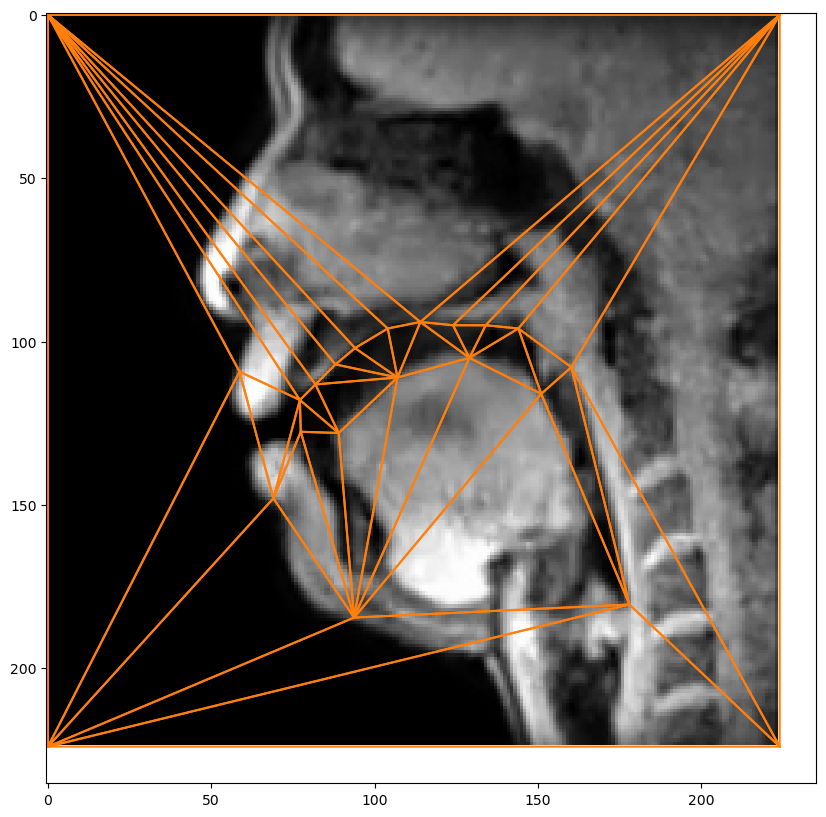
\includegraphics[height=0.7\textheight]{triangles.png}}
\end{frame}

\begin{frame}
  \frametitle{Once you have drawn the triangles, they move along with the points}
  \centerline{\animategraphics[loop,controls,height=2.5in]{20}{exp/mp1_procrustes_triangles-}{0}{42}}
\end{frame}


%%%%%%%%%%%%%%%%%%%%%%%%%%%%%%%%%%%%%%%%%%%%%%%%%%%%%%%%%
\section[Barycentric coordinates]{Step 4: Find the mapping between original and moved pixels: Barycentric coordinates}
\setcounter{subsection}{1}

\begin{frame}
  \begin{columns}[t]
    \column{2.5in}
    \begin{block}{Source image}
      The source image is divided into non-overlapping triangles, $X_k$.
      \centerline{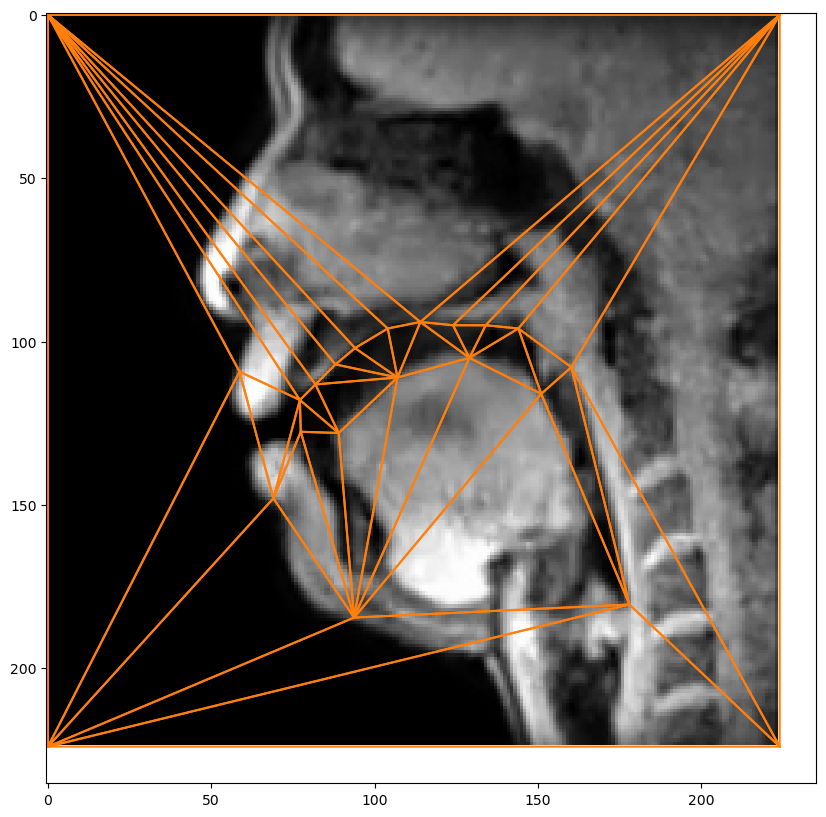
\includegraphics[width=\textwidth]{triangles.png}}
    \end{block}
    \column{2.25in}
    \begin{block}{Target image}
      In the target image, those triangles have moved to new locations, $Y_k$.
      \centerline{\animategraphics[loop,controls,width=\textwidth]{20}{exp/mp1_procrustes_triangles-}{0}{42}}
    \end{block}
  \end{columns}
\end{frame}  

\begin{frame}
  \frametitle{Problem Statement: Moving pixels}

  \begin{itemize}
  \item
    The size of the image we want to construct is $m\times n$.
  \item
    Consider a particular augmented target pixel,
    $y=\left[\begin{array}{c}y_1\\y_2\\1\end{array}\right]$, where $0\le
    y_1\le m-1$ and $0\le y_2\le n-1$ are both integers.
  \item
    In order to find the color of target pixel $y$, we want to find
    out which source pixel, $x$, was moved to that location.  Assume
    that pixels only move around -- they don't change color while they
    move.
  \end{itemize}
\end{frame}
\begin{frame}
  \frametitle{Problem Statement: Piece-wise affine transform}

  \begin{itemize}
  \item
    Suppose that $y\in Y_k$, the $k^{\text{th}}$ target
    triangle.
  \item
    We know therefore that $x\in X_k$.  But there are lots
    of pixels inside $X_k$.  Which one is it?
  \item
    Let's assume that, within each triangle, the pixels move according
    to an affine transform.  In other words, if $y\in Y_k$,
    and if we already knew $A_k$, then we could find $x$ by solving:
    \begin{displaymath}
      y = A_k x
    \end{displaymath}
    where
    \[
    y=\left[\begin{array}{c}y_1\\y_2\\1\end{array}\right],~~~
    x=\left[\begin{array}{c}x_1\\x_2\\1\end{array}\right],~~~
    A_k=\left[\begin{array}{ccc}a_{1,1}&a_{1,2}&a_{1,3}\\a_{2,1}&a_{2,2}&a_{2,3}\\0&0&1\end{array}\right]
    \]
  \end{itemize}
\end{frame}

\begin{frame}
  \frametitle{Piece-wise affine transform}
  \[
  \mbox{target point:}~y=\left[\begin{array}{c}y_1\\y_2\\1\end{array}\right],~~~
  \mbox{source point:}~x=\left[\begin{array}{c}x_1\\x_2\\1\end{array}\right]
  \]
  {\bf Definition}: if $y$ is in the $k^{\textrm{th}}$ triangle in the
  {\bf output image}, then we want to use the $k^{\textrm{th}}$ affine
  transform:
  \[
  y=A_k x,~~~x=A_k^{-1}y
  \]
\end{frame}

\begin{frame}
  If {\bf it is known that} $x=A_k^{-1}y$ for some unknown
  affine transform matrix $A_k$,
  \vspace*{2mm}\\
  then
  \vspace*{2mm}\\
  the method of barycentric
  coordinates finds $x$
  \vspace*{2mm}\\
  {\bf without ever finding} $A_k$.
\end{frame}

\begin{frame}
  \begin{columns}[t]
    \column{2.5in}
    \begin{block}{Barycentric Coordinates}
    Barycentric coordinates turns the problem on its head.  Suppose
    $y$ is in a triangle with corners at $y_1$,
    $y_2$, and $y_3$. That means that
    \[
    y=\beta_1y_1+\beta_2y_2+\beta_3y_3
    \]
    where
    \[
    0\le \beta_1,\beta_2,\beta_3\le 1
    \]
    and
    \[
    \beta_1+\beta_2+\beta_3=1
    \]
    \end{block}
    \column{2.25in}
    \begin{block}{}
      \centerline{\includegraphics[width=2.25in]{exp/Barycentric.png}}
    \end{block}
  \end{columns}
\end{frame}

\begin{frame}
  \frametitle{Barycentric Coordinates}
  Suppose that all three of the corners are 
  transformed by some affine transform $A$, thus
  \[
  x_1=Ay_1,~~
  x_2=Ay_2,~~
  x_3=Ay_3
  \]
  Then if
  \[
  \mbox{If:}~y=\beta_1y_1+\beta_2y_2+\beta_3y_3
  \]
  Then:
  \begin{eqnarray*}
    x &=& Ay\\
    &=& \beta_1Ay_1+\beta_2Ay_2+\beta_3Ay_3\\
    &=& \beta_1x_1+\beta_2x_2+\beta_3x_3
  \end{eqnarray*}
  In other words, once we know $\beta$, we no longer need to
  find $A$.  We only need to know where the corners of the triangle
  have moved.
\end{frame}

\begin{frame}
  \begin{columns}[t]
    \column{2.5in}
    \begin{block}{Barycentric Coordinates}
      If
      \[
      y=\beta_1y_1+\beta_2y_2+\beta_3y_3
      \]
      Then
      \[
      x= \beta_1x_1+\beta_2x_2+\beta_3x_3
      \]
    \end{block}
    \column{2.25in}
    \begin{block}{}
      \centerline{\includegraphics[width=2.25in]{exp/Barycentric.png}}
    \end{block}
  \end{columns}
\end{frame}

\begin{frame}
  \frametitle{How to find Barycentric Coordinates}
  But how do you find $\beta_1$, $\beta_2$, and $\beta_3$?
  \[
  \left[\begin{array}{c}y_1\\y_2\\1\end{array}\right]=
  \beta_1y_1+\beta_2y_2+\beta_3y_3
  =\left[\begin{array}{ccc}y_{1,1}&y_{1,2}&y_{1,3}\\y_{2,1}&y_{2,2}&y_{2,3}\\1&1&1\end{array}\right]
  \left[\begin{array}{c}\beta_1\\\beta_2\\\beta_3\end{array}\right]
  \]
  Write this as:
  \[
  y=Y\beta
  \]
  Therefore
  \[
  \beta = Y^{-1}y
  \]
  This {\bf always works:} the matrix $Y$ is always invertible, unless
  all three of the points $y_1$, $y_2$, and $y_3$
  are on a straight line.
\end{frame}
\begin{frame}
  \frametitle{How do you find out which triangle
    the point is in?}
  \begin{itemize}
  \item Suppose we have $K$ different triangles, each of which is
    characterized by a $3\times 3$ matrix of its corners
    \[
    Y_k = \left[y_{1}^{(k)},y_{2}^{(k)},y_{3}^{(k)}\right]
    \]
    where $y_{m}^{(k)}$ is the $m^{\textrm{th}}$ corner of the
    $k^{\textrm{th}}$ triangle.
  \item Notice that, for any point $y$, for ANY triangle $Y_k$,
    we can find
    \[\beta = Y_k^{-1}y\]
  \item However, the coefficients $\beta_1$, $\beta_2$, and
    $\beta_3$ will all be between $0$ and $1$ {\bf if and only if}
    the point $y$ is inside the triangle $Y_k$.  Otherwise, some
    of the elements of $\beta$ must be negative.
  \end{itemize}
\end{frame}

\begin{frame}
  \frametitle{The Method of Barycentric Coordinates}
  To construct the animated output image frame $J[y_2,y_1]$, we do
  the following things:
  \begin{itemize}
  \item First, for each of the reference triangles $X_k$ in the input
    image $I(x_2,x_1)$, decide where that triangle
    should move to.  Call the new triangle location $Y_k$.
  \item Second, for each integer output pixel $(y_1,y_2)$:
    \begin{itemize}
    \item For each of the triangles, find $\beta=Y_k^{-1}y$.
    \item Choose the triangle for which all of the elements of $\beta$
      are $0\le\beta_m\le 1$.
    \item Find $x=X_k\beta$.
    \item Find the color of pixel $I(x_2,x_1)$ in the input image.
    \item Set $J[y_2,y_1]=I(x_2,x_1)$.
    \end{itemize}
  \end{itemize}
\end{frame}


%%%%%%%%%%%%%%%%%%%%%%%%%%%%%%%%%%%%%%%%%%%%%%%%%%%%%%%%%
\section[Image interpolation]{Step 5: Find the color of the source pixel: Bilinear interpolation}
\setcounter{subsection}{1}

\begin{frame}
  \begin{block}{Integer Target Points}
    Now let's suppose that you've figured out the coordinate transform:
    for any given $J[y_2,y_1]$, you've figured out which pixel should be used to create it 
    ($J[y_2,y_1]=I(x_2,x_1)$).
    \begin{displaymath}
      x=X_k\beta=X_kY_k^{-1}y
    \end{displaymath}
  \end{block}
  \begin{block}{The Problem: Non-Integer Input Points}
    If $[y_2,y_1]$ are integers, then usually, $(x_2,x_1)$ are not integers.
  \end{block}
\end{frame}

\begin{frame}
  \frametitle{Image Interpolation}

  It is necessary to find $I(v,u)$ at non-integer values of $(v,u)$ by
  interpolating between the integer-valued pixels provided in the image file. 

  Given the pixels of $I[n,m]$ at integer values of $m$ and $n$, we
  can interpolate using an interpolation kernel $h(v,u)$:
  \[
  I(v,u) = \sum_m\sum_n I[n,m] h(v-n,u-m)
  \]
\end{frame}

\begin{frame}
  \frametitle{Piece-Wise Constant Interpolation}
  \begin{equation}
  I(v,u) = \sum_m\sum_n I[n,m] h(v-n,u-m)
  \label{eq:interpolation1}
  \end{equation}
  For example, suppose
  \[
  h(v,u) = \left\{\begin{array}{ll}
  1 & 0\le u<1,~~0\le v<1\\
  0 & \mbox{otherwise}
  \end{array}\right.
  \]
  Then Eq. (\ref{eq:interpolation1}) is the same as just truncating $u$
  and $v$ to the next-lower integer, and outputting that number:
  \[
  I(v,u) = I\left[\lfloor v\rfloor,\lfloor u\rfloor\right]
  \]
  where $\lfloor u\rfloor$ means ``the largest integer smaller than $u$''.
\end{frame}

\begin{frame}
  \frametitle{Example: Original Image}
  For example, let's downsample this image, and then try to recover it by image interpolation:
  \centerline{\includegraphics[width=4.5in]{exp/original.png}}
\end{frame}

\begin{frame}
  \frametitle{Example: Downsampled Image}
  Here's the downsampled image:
  \centerline{\includegraphics[width=4.5in]{exp/downsampled.png}}
\end{frame}

\begin{frame}
  \frametitle{Example: Upsampled Image} Here it is after we upsample
  it back to the original resolution (insert 3 zeros between every
  pair of nonzero columns):
  \centerline{\includegraphics[width=4.5in]{exp/upsample.png}}
\end{frame}

\begin{frame}
  \frametitle{Example: PWC Interpolation}

  Here is the piece-wise constant interpolated image:
  \centerline{\includegraphics[width=4.5in]{exp/pwc.png}}
\end{frame}

\begin{frame}
  \frametitle{Bi-Linear Interpolation}
  \[
  I(v,u) = \sum_m\sum_n I[n,m] h(v-n,u-m)
  \]
  For example, suppose
  \[
  h(v,u) = \max\left(0,(1-|u|)(1-|v|)\right)
  \]
  Then Eq. (\ref{eq:interpolation1}) is the same as piece-wise linear
  interpolation among the four nearest pixels.  This is called {\bf
    bilinear interpolation} because it's linear in two directions.
  \begin{align*}
    m &= \lfloor u\rfloor,~~~e=u-m\\
    n &= \lfloor v\rfloor,~~~f=v-m\\
    I(v,u) &= (1-e)(1-f)I[n,m]+(1-e)fI[n,m+1]\\
    &+e(1-f)I[n+1,m]+efI[n+1,m+1]
  \end{align*}
\end{frame}

\begin{frame}
  \frametitle{Example: Upsampled Image}

  Here's the upsampled image again:
  \centerline{\includegraphics[width=4.5in]{exp/upsample.png}}
\end{frame}

\begin{frame}
  \frametitle{Example: Bilinear Interpolation}

  Here it is after bilinear interpolation:
  \centerline{\includegraphics[width=4.5in]{exp/pwl.png}}
\end{frame}


\begin{frame}
  \frametitle{PWC and PWL Interpolator Kernels}

  Bilinear interpolation uses a PWL interpolation kernel, which does
  not have the abrupt discontiuity of the PWC interpolator kernel.
  \centerline{\includegraphics[width=4.5in]{exp/interpolators.png}}
\end{frame}


\begin{frame}
  \frametitle{Sinc Interpolation}
  \[
  I(v,u) = \sum_m\sum_n I[n,m] h(v-n,u-m)
  \]
  For example, suppose
  \[
  h(v,u) = \mbox{sinc}(\pi u)\mbox{sinc}(\pi v)
  \]
  Then Eq. (\ref{eq:interpolation1}) is an ideal band-limited sinc interpolation.
  It guarantees that the continuous-space image, $I(v,u)$, is exactly a band-limited
  D/A reconstruction of the digital image $I[n,m]$.
\end{frame}

\begin{frame}
  \frametitle{Sinc Interpolation}

  Here is the cat after sinc interpolation:
  \centerline{\includegraphics[width=4.5in]{exp/sincinterp.png}}
\end{frame}


\begin{frame}
  \frametitle{Summary of interpolation methods}

  \begin{itemize}
  \item PWC interpolation results in a blocky image
  \item Sinc interpolation results in a smooth image, and would be
    perfect if the input image was infinite in size, but since
    real-world images have edges, the sinc interpolation produces
    ripple artifacts
  \item Bilinear interpolation is a very efficient solution with good results
  \item Better results are available using deep-learning-based
    super-resolution neural nets, but only after the neural net has
    been trained for a few weeks!
  \end{itemize}
\end{frame}

%%%%%%%%%%%%%%%%%%%%%%%%%%%%%%%%%%%%%%%%%%%%%%%%%%%%%%%%%
\section{Conclusion}
\setcounter{subsection}{1}

\begin{frame}
  \frametitle{Strategy}
  \begin{enumerate}
  \item Use MMSE affine projection to rotate, scale, and shear the XRMB
    points so that they match the shape of the MRI as well as possible.
  \item Draw triangles on the MRI so that every pixel is inside a triangle.
  \item Move the triangles.
  \item Map each integer pixel in the target image to a real-valued pixel in the original image
    using barycentric coordinates
  \item Use bilinear interpolation to find the color of the pixel 
  \end{enumerate}
\end{frame}

\end{document}

